\section{模型检验与实验结果}
\subsection{数据来源与统计口径}
对单案例定义 $\eta=N_c/N_{\rm true}$、$\bar t=T/N_c$，其中 $N_c=0$ 时每源时间未定义，应记录失败。源总数只在测试结束后用于评价，不作为策略的在线输入。跨案例报告全清案例数及逐案例 $\bar t$ 的中位数，不能用 $\sum T/\sum N_c$ 替代该中位数。

本文使用三类证据：最终参数下重新执行的第三问本地消融；仓库保留的第四问逐案例复核JSON及布局证书；官方模拟器两场演练的记录。正式测试另列。旧版失败清除按5秒计算的历史成绩不纳入主表，主表统一使用失败3秒、成功5秒。源位置和方向真值仅用于离线校验。

\subsection{第三问：布局、路由与覆盖清除的消融}
固定模拟器、种子和计时，分别改变布局、or-opt及覆盖清除。布局记为“环顶点数/环半径/每频道扫描读数上限”。各臂在三个种子集上均全清，结果见表\ref{tab:q3ablation}。种子1至30是1至60的子集，不能将两组样本量相加视为独立案例。
\begin{table}[htbp]\centering\small
\caption{第三问最终配置消融：每源时间中位数（秒/源）}\label{tab:q3ablation}
\begin{tabular}{lrrr}\toprule
方法&种子1--30&种子1--60&种子61--160\\\midrule
v8基线&265.92&278.10&278.02\\
v15旧布局，or-opt关&272.41&281.94&279.29\\
v15最终布局，or-opt关&263.81&277.46&278.74\\
v15最终布局，or-opt开&256.68&275.51&271.65\\
v18最终布局，or-opt关&263.24&277.45&278.74\\
v18最终版&256.11&275.54&272.08\\
\bottomrule\end{tabular}
\end{table}
固定or-opt关闭时，布局从7/1110/2改为6/1130/3，三组分别降低8.60、4.48、0.55秒/源；固定最终布局时，开启or-opt分别降低7.13、1.95、7.09秒/源。可见布局收益随案例集变化，不能把不同因素合并归因。

在已开启or-opt的条件下，覆盖式清除相对上一臂的变化为 $-0.57,+0.03,+0.43$ 秒/源，接近中性。采用统一覆盖机制主要为了清除可靠性，而非宣称其在全向场景显著加速。种子61至160中，最终版相对v8的每源时间中位数下降约2.13\%；这是中位数之间的比较，不代表每个案例均下降2.13\%。

\subsection{第四问：发现与清除可靠性}
对默认混合与全定向压力场景，分别使用三个互不重叠的种子段。v14采用较早发现与射线清除机制，v17换成24点布局并增加小环试清，v18增加知识矩阵失败圆与覆盖清除。各方法在同一场景、同一种子下使用相同源配置。
\begin{table}[htbp]\centering\small
\caption{第四问全清案例数与最终版每源时间中位数}\label{tab:q4audit}
\begin{tabular}{llrrrr}\toprule
种子段&场景&v14&v17&v18&v18秒/源\\\midrule
1--60&混合&57/60&60/60&60/60&487.24\\
1--60&全定向&53/60&57/60&60/60&580.73\\
61--160&混合&94/100&97/100&100/100&488.75\\
61--160&全定向&85/100&97/100&100/100&560.44\\
161--260&混合&95/100&98/100&100/100&486.13\\
161--260&全定向&86/100&96/100&100/100&553.15\\
合计&两场景&470/520&505/520&520/520&---\\
\bottomrule\end{tabular}
\end{table}
最终版在520个本地案例中清除6684/6684个源。v17共505/520局全清，v18补齐其15个未全清案例。两个场景复用种子编号，但场景的发射方向构成不同，因此这里计为520个“种子与场景”的组合，不能解释为520次官方测试。

失败记录揭示修复对象：混合场景种子80、频道19的估计误差约33.3米，旧六点环最近试清点仍距真源21.51米；全定向种子128、频道11曾在距真源15.9米处因波束背面返回无信号，射线距离判断随后偏离。二者均已被发现，说明发现完备不等于清除完备。25米格覆盖使用原保守域和方向无关的失败圆，针对这一问题提供最终补救。
\begin{figure}[htbp]\centering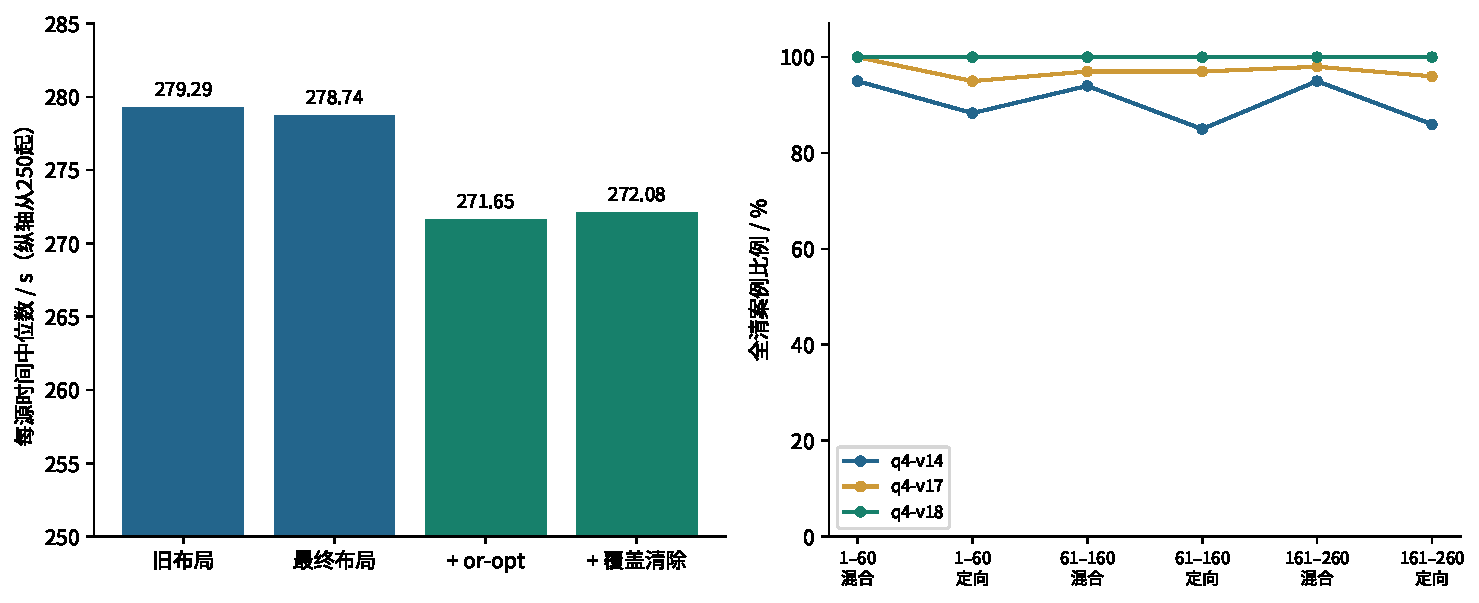
\includegraphics[width=.96\linewidth]{figures/ablation.pdf}
\caption{左：第三问种子61至160的消融；右：第四问六组场景的全清比例。图表来自本地模拟记录。}\end{figure}

\subsection{官方模拟器演练}
2026年9月13日14:19至14:23的两局演练分别使用最终入口 \texttt{q3-v18}、\texttt{q4-v18}，结果记录于支撑材料 \texttt{official-drill-20260913-1420-q18.json}。源总数来自官方测试结束后的结果记录；问题四包含4个全向源及11个定向源。
\begin{table}[htbp]\centering\small
\caption{官方演练结果（每问一场，非正式测试）}
\begin{tabular}{lrr}\toprule
指标&问题三&问题四\\\midrule
案例编码&\texttt{VSSN-5G4G-AWMY-2ENJ}&\texttt{2FAE-SPSW-TG7E-UQH3}\\
清除个数/总数&14/14&15/15\\
清除比例&100\%&100\%\\
虚拟总时间（秒）&3357.525&6339.556\\
平均定位清除时间（秒/源）&239.82&422.64\\
检测次数&110&240\\
清除尝试次数（失败次数）&19（5）&16（1）\\
记录的程序运行时间（秒）&0.5&0.6\\\bottomrule
\end{tabular}\end{table}
两场演练支持最终程序在官方环境中可运行且在对应案例中全清。每问只有一个案例，不能估计稳定的成功率或断言优于另一策略；程序运行时间按现有记录精度保留。官方案例分布、通信和计时环境与本地模拟不同，不直接合并统计。
\placeholder{官方演练代表性轨迹与结果界面}{补充上述两场官方演练的轨迹或Q2回放界面截图，保留案例编码，标出扫描停点、清除位置、虚拟时间和最终清除个数。使用真实导出或回放，不将几何示意图当作实测轨迹。}

\subsection{问题三正式测试结果}
\begin{table}[htbp]\centering\small
\caption{问题三正式测试结果}
\begin{tabular}{llll}\toprule
测试案例编码&清除干扰源个数&平均定位清除时间&程序运行时间\\\midrule
{[正式测试1编码]}&[待填]&[待填，秒/源]&[待填，秒]\\
{[正式测试2编码]}&[待填]&[待填，秒/源]&[待填，秒]\\
{[正式测试3编码]}&[待填]&[待填，秒/源]&[待填，秒]\\\bottomrule
\end{tabular}\end{table}
\subsection{问题四正式测试结果}
\begin{table}[htbp]\centering\small
\caption{问题四正式测试结果}
\begin{tabular}{llll}\toprule
测试案例编码&清除干扰源个数&平均定位清除时间&程序运行时间\\\midrule
{[正式测试1编码]}&[待填]&[待填，秒/源]&[待填，秒]\\
{[正式测试2编码]}&[待填]&[待填，秒/源]&[待填，秒]\\
{[正式测试3编码]}&[待填]&[待填，秒/源]&[待填，秒]\\\bottomrule
\end{tabular}\end{table}
[按每问三次正式测试的官方结果填写以上两表，并将六份官方导出日志以原文件名放入支撑材料。当前可核验记录为演练，不替代正式结果。]

\section{模型评价与改进方向}
本模型将不确定位置表示为可行集，使测向误差界直接参与定位，并区分直径与包围半径。知识矩阵使多类反馈可追溯，联合调度减少扫描与清除的重复移动；局部凸包判据将未知朝向的半圆发现转化为有限几何检验；覆盖式清除利用与方向无关的光学反馈弥补定向背面难题。

模型仍有三方面边界。其一，滚动路由和估计点试清属于启发式，不保证全局最短耗时，负观测修正质心也不保证每个案例都更快。其二，数值外包络、凸包容差及退化区域会影响实现，连续单元证书尚非区间算术证明。其三，64格和执行预算使理论覆盖命题具有执行前提，当前全清结果只能说明所测案例成功，不能消除所有未测情形的风险。

后续可在保持保守域的前提下，对未完成覆盖计划分批续接，保留更完整的负证据事件表，并以同分布、多场官方演练评估稳定性。对当前交付而言，报告实际成功反馈、保存原始日志、区分本地与官方统计，是保证结论可核验的必要条件。
